\section{Hardware Design Choices}

\subsection{Providing Test Data}
In order for the driver to stress the DUT, the verification system must perform at a much higher frequency than the expected frequency of the DUT.
Assuming the DUT is to run at 300MHz, to fully explore the effect of overclocking, the testbench must be able to run at double the frequency.
This gives an ambitious target frequency of 800MHz.
Assuming a data width of 32-bit, the target data transfer rate is then estimated to be 25.6Gbps.
With this rough estimate, we can start considering different design options.

\subsubsection{HPS-FPGA Bridge}
As the testing is to be controlled by the HPS, the HPS-FPGA bridge will be the immediate bottleneck if the test data is to flow from HPS to FPGA.
While the HPS can easily generate test data with a piece of software, there is a large amount of overhead as data crosses from one architecture to another.
This overhead exists in the form of both decreased bandwidth and increased delay.
Thus, it is not be sensible for the HPS to send out data during runtime.

\subsubsection{Off-chip DDR SDRAM}
Another thought may be to first populate the off-chip DDR SDRAM on the FPGA side, then feed that data to the DUT during test.
This is already much faster than passing the data directly from HPS.
The 1GB, 32-bit wide DDR3 on the FPGA side is rated at 400MHz.
With double rate transfer, this gives a maximum transfer rate of 25.6Gbps.

Although using the off-chip RAM may theoretically achieve the targets, it still has its disadvantages.
Firstly, the process of filling up the memory takes time.
Thus, the testing would be broken up into bursts, with time in between for checking results and filling in new data.
The complexity of the SDRAM interface also requires an SDRAM controller to be used to manage SDRAM refresh cycles, address multiplexing and interface timing.
These all add up to significant access latency.
While it could be overcome with burst and piplined accesses, it would further complicate the SDRAM controller.
A controller is provided by Intel~\cite{Altera3}, but it would consume a non-negligible amount of the limited FPGA resources while adding unnecessary complexities to the design.
Customising or building a new SDRAM controller to fit this project is possible, but needlessly time-consuming.

\subsubsection{On-chip Memory}
The on-chip memory is much faster and simpler to use.
In comparison, this memory is implemented on the FPGA itself, and thus needs no external connections for accesses.
It has higher throughput and lower latency than the SDRAM.
The memory transactions can also be piplined, giving one transaction per clock cycle.
With an on-chip FIFO accessed in dual-port mode, the write operations at one end and the read operations at the other end can happen simultaneously.
This feature is useful as tests are prepared and fed into the DUT, or when test results are collected and fed to the monitor.

On-chip memory is not without its drawbacks.
It is volatile like SDRAM and very limited in capacity.
SDRAMs can have store about 1GB, while on-chip memory could only hold a few MB~\cite{Altera2}.
Volatility is not exactly of concern in this project, but its small capacity means not much test data can be held before it needs more fed in.

\subsubsection{Distributed RAM / Registers}
On-chip memory has a minimum latency of 1 clock cycle as the R/W access gets processed.
If a even faster memory is desired, we can use LUTs or registers to store them.
This option would eliminate the latency but takes up much more FPGA resources.
The capacity is even more limited as LUTs are usually used for logic.
There will be a significant amount of data generated during testing, and the testbench should be as lightweight as possible to allow flexibility in the DUTs.
As such, distributed RAM will not be used in this project for data transfer.
Registers will still be used as they are essential for many other purposes.

\subsubsection{Real Time Data Generation}
As seen from the analysis, the best design option here should be able to exploit the benefits of on-chip memory, and circumvent the drawback of buffering testing data generated from the HPS.
Generating testing data at runtime, on the FPGA will be such a method.
As arithmetic operators have a vast set of valid inputs, it is necessary to have cost-effective test generation.

A good choice here is to use random testing.
With relatively low effort, random testing can provide significant coverage and discover relatively subtle errors~\cite{Duran1}.
The main drawback of random testing is the possible lack of coverage for corner cases, for which the usual solution is to provide handwritten tests to complement it.
However, as the main goal of this testbench is gauging the performance of the module, and not necessarily verifying the correctness of the module, having uncovered testing holes is acceptable during stress testing.
As the project progress, special tests could be written and run separately with a relaxed timing restriction to cover the holes.
It should be noted that certain corner cases may represent critical paths in the design.
To combat this, the testbench provides the option to run handwritten inputs alongside random tests.

\subsection{LFSR Randomiser}

LFSRs are a reliable way of generating pseudorandom numbers quickly with low cost~\cite{Hazwani1}.
Fulfilling the design requirements, they will thus form the starting point of data generation.
While it is possible for data generated to be invalid as inputs to the DUT, this should not be the case for most arithmetic units.
Even if this is the case, they can be dealt by the filter in the driver.

Following this approach, the software would only need to configure the generation at the beginning, and test data no longer needs to pass through the HPS-FPGA bridge.
Thus, the testbench can provide fast and constant data to stress the DUT.

\subsubsection{LFSR Configurations}

While LFSRs are simple hardware modules, there are still a few design options we should explore before implementing them.
To compare, we can examine an 8-bit LFSR with taps on bit [7,5,4,3].

In a Fibonacci LFSR, the taps are pulled and fed into a cascade of XOR gates.
The output of the final XOR gate is then the lowest bit of the next random number.
The higher bits are obtained by one left bitwise shift.

\begin{figure}[ht]
  \centering
  \begin{tikzpicture}
  [
    x=1em, y=1em,
    start chain = going right,
    node distance = 0em,
    reg/.style =
      {draw, minimum width=2em, minimum height=2em,outer sep=0pt, on chain},
    every join/.style={-, thick}
  ]
  \node [reg] at (0, 0) (1) {1};
  \node [reg] (2) {};
  \node [reg] (3) {};
  \node [reg] (4) {4};
  \node [reg] (5) {5};
  \node [reg] (6) {6};
  \node [reg] (7) {};
  \node [reg] (8) {8};

  \node[xor gate US,draw,rotate=180] at (2.5, 2) (a) {};
  \node[xor gate US,draw,rotate=180] at (5.5, 3) (b) {};
  \node[xor gate US,draw,rotate=180] at (8.5, 4) (c) {};

  \draw (4.north)  |- (a.input 1);
  \draw (5.north)  |- (b.input 1);
  \draw (6.north)  |- (c.input 1);

  \draw (b.output) to[-|-] (a.input 2);
  \draw (c.output) to[-|-] (b.input 2);
  \draw (8.north)       |- (c.input 2);

  \draw (a.output) -- (-2, 2) |- (1.west);

\end{tikzpicture}
  \caption{Fibonacci Configuration}
  \label{FibLFSR}
\end{figure}

In a Galois LFSR, the new bits in the taps are obtained by a XOR operation between the lowest bit and the bit on the left of each tap.
The highest bit is simply the previous lowest bit, and all other bits are obtained by one right bitwise shift.

\begin{figure}[ht]
  \centering
  \begin{tikzpicture}
  [
    x=1em, y=1em,
    start chain = going right,
    node distance = 0em,
    reg/.style =
      {draw, minimum width=2em, minimum height=2em, outer sep=0pt, on chain},
    spa/.style =
      {minimum width=3em, minimum height=2em, outer sep=0pt, on chain},
    every join/.style={-, thick}
  ]
  \node [reg] at (0, 0) (1) {1};
  \node [reg] (2) {};
  \node [reg] (3) {};
  \node [reg] (4) {4};
  \node [spa] ()  {};
  \node [reg] (5) {5};
  \node [spa] ()  {};
  \node [reg] (6) {6};
  \node [spa] ()  {};
  \node [reg] (7) {};
  \node [reg] (8) {8};

  \node[xor gate US,draw,rotate=180] at  (8.5, 0) (a) {};
  \node[xor gate US,draw,rotate=180] at (13.5, 0) (b) {};
  \node[xor gate US,draw,rotate=180] at (18.5, 0) (c) {};

  \draw (1.west) -| (-2, -2) -- (25,-2) |- (8.east);

  \draw  (9.7,-2) |- (a.input 1);
  \draw (14.7,-2) |- (b.input 1);
  \draw (19.7,-2) |- (c.input 1);

  \draw (a.input 2-|5.west) -- (a.input 2);
  \draw (b.input 2-|6.west) -- (b.input 2);
  \draw (c.input 2-|7.west) -- (c.input 2);

  \draw (a.output) -- (4.east);
  \draw (b.output) -- (5.east);
  \draw (c.output) -- (6.east);

\end{tikzpicture}
  \caption{Galois Configuration}
  \label{GalLFSR}
\end{figure}

Other LFSR configurations such as Xorshift~\cite{Marsaglia1} exists, but they are mostly designed and optimised as pieces of software, thus being less appropriate for this design.



\subsubsection{Randomiser Structure}

\textit{Horizontal} --
Easy to build, easy to test with.

\begin{figure}[ht]
  \centering
  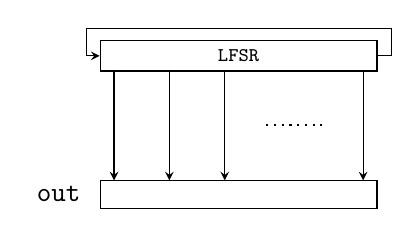
\begin{tikzpicture}
  [
    x=1em, y=1em
  ]
  \node at (-1.5, 0) {\texttt{out}};
  \node [draw,minimum height=1em, minimum width=10em] at (5, 0) (o) {};
  \node [draw,minimum height=1em, minimum width=10em] at (5, 5) (1) {\scriptsize \texttt{LFSR}};
  \draw [->, >=stealth] (1.east) -| ++(0.5, 1) -- ++(-11, 0) |- (1.west);
  \foreach \pos [count=\idx] in {0.5, 2.5, 4.5, 9.5}{
    \draw [->, >=stealth] (\pos, 4.5) -- (\pos, 0.5);
  }
  \draw [dotted, thick] (6, 2.5) -- (8, 2.5);

\end{tikzpicture}
  \caption{Horizontal Structure}
  \label{HoriLFSR}
\end{figure}

\textit{Vertical} --
Nice randomness, more scalable, need to seed all the LFSRs differently.

\begin{figure}[ht]
  \centering
  \begin{tikzpicture}
  [
    x=1em, y=1em
  ]
  \node at (-1.5, 0) {\texttt{out}};
  \node [draw,minimum height=1em, minimum width=10em] at (5, 0) (o) {};
  \foreach \pos [count=\idx] in {0.5, 2.5, 4.5, 9.5}{
    \node [draw,minimum height=1em, minimum width=5em, rotate around={90:(0, 0)}] at (\pos, 5) (\idx) {\scriptsize \texttt{LFSR}};
    \draw [->, >=stealth] (\idx.west) -- (\idx.west|-o.north);
    \draw [->, >=stealth] ($(\idx.west)-(0, 0.5)$) -| (\pos-1,8) -| (\idx.east);
  }

  \draw [dotted, thick] (6, 5) -- (7.5, 5);

\end{tikzpicture}
  \caption{Vertical Structure}
  \label{VertLFSR}
\end{figure}

\subsection{Driver}
\subsubsection{Dual Driver System}
One driver focusses on fast stress tests, The other allows handwritten tests to coexist with random tests.
They can be switched in software.

\subsection{Monitor}

Another concern in the system design is of the different clock domains that must exist on the FPGA.
At a minimum, there need to be two clock domains: one surrounds the DUT and another supports the rest of the control logic around the DUT.
These clock frequencies can be generated with PLLs, which are provided as IP Cores in the Quartus software~\cite{Altera4}.
A clock tree will distribute them to the individual modules.
Data crossing clock domains will be fed through FIFOs to prevent loss.

The proposed structure will have the bulk of the control logic running in a separate clock domain to the DUT.
Only an interface with FIFOs will be running in synchronicity with the DUT.
Therefore, the test controls can run at a slower frequency without bottlenecking the system, allowing the DUT to be stressed further.
The problem now is to ensure the monitor can handle the stream of DUT output coming in at a higher frequency that it is running at.
As the monitor needs to calculate the correct data before it can check if the DUT output is correct, it cannot keep up with the speed of the DUT.
This report consider three alternatives.

\subsubsection{Partial Monitors}
A lightweight idea is to implement a parity checker instead of a full model inside the monitors.
For example, to check an adder, the monitor can just check if the final bit with a LUT acting as a XOR gate.

Although this is reasonably fast, it cannot be extended once the DUT is faster than a parity calculation followed by a comparison.
More critically, it provides no additional information once the DUT fails, and it has a 50\% rate of ignoring an error.
If this is to be solved by increasing the number of bits checked, the problem returns back to its initial state.
Thus this method will not be experimented.

\subsubsection{Lazy Monitors}

\begin{figure}[H]
  \centering
  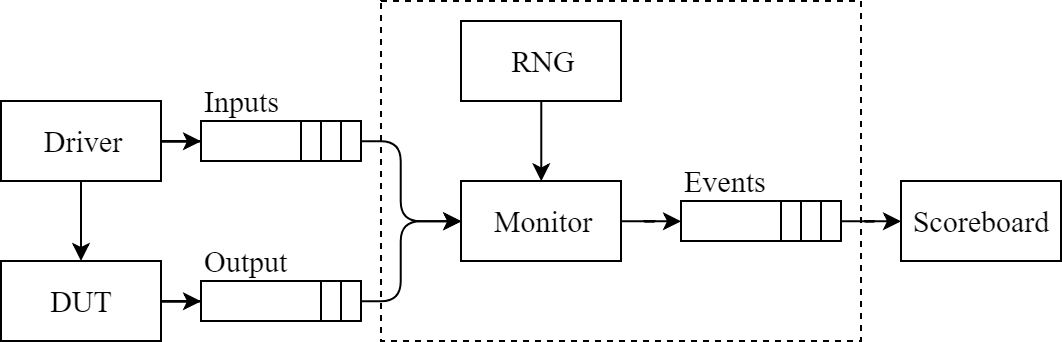
\includegraphics[width=12cm]{img/LazMon}
  \caption{Structure of a Lazy Monitor}
  \label{LazMon}
\end{figure}

An more scalable alternative is to have the monitor only check a selection of data sets.
For example, if the monitor is programmed to check every third test point, statistically it will make little difference to the final result.
In case the DUT is aware of this and only produce correct outputs on every third operation, this process can be randomised too.

This method can be extended if the DUT get fast simply by skipping more checks, and it has the full information when it detects an error.
However, this method needs the extra logic in the random controller, making the monitor slightly more complex than it probably should be.

\subsubsection{Parallel Monitors}

\begin{figure}[H]
  \centering
  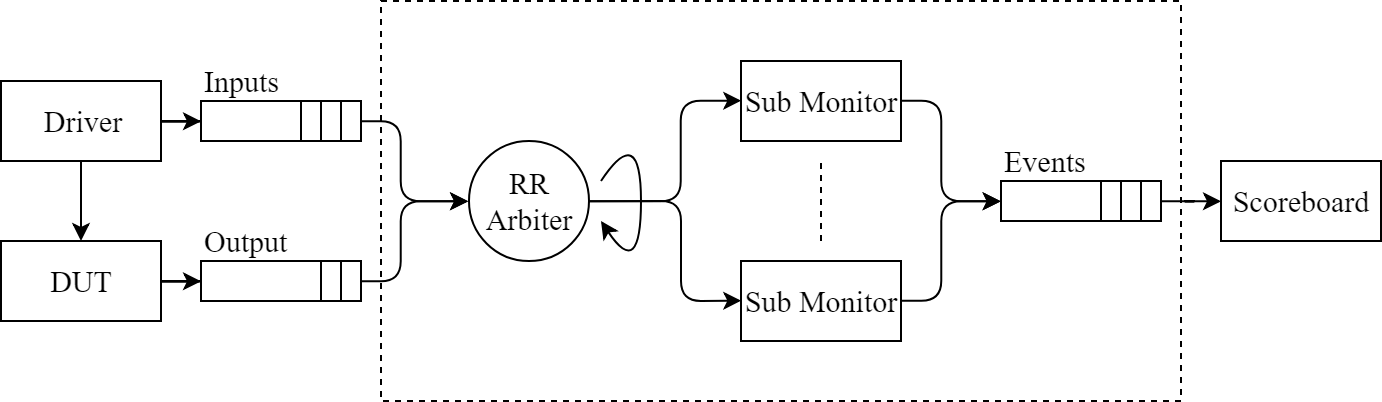
\includegraphics[width=15cm]{img/ParMon}
  \caption{Structure of a Parallel Monitor}
  \label{ParMon}
\end{figure}

As the test data is uniform, the monitor can be parallelised in to a number of sub-monitors.
The sub-monitors is connected to a arbiter that is connected to three FIFOs.
The FIFOs are the inputs and the output of the DUT.
A round robin arbiter distributes the data to the sub-monitors equally.
The results from each sub-monitor are then sent to a single scoreboard.
To avoid potential hazards, the output from the sub-monitors will be buffered before processed by the scoreboard.

This does not have data dependency on a random controller, and it can fully guarantee the correctness of the DUT.
It is also scalable as more sub-monitors can be added it the DUT fills up its output buffer.
As a downside, this method takes up the most FPGA resources to implement as it scales.

Comparing across the three methods, the parallel monitors will be built first for this project, as it offers the best functionalities.
Although unlikely, if a fatal issue arises in this design, or if the testbench needs to be more lightweight, then the lazy monitor will be used as the alternative.

\subsection{Scoreboard}

If the monitor detects an interesting event such as an error, it will send a message to the scoreboard.
The scoreboard has counters tracking these events, which are exposed and can be read by the HPS.

The software can run statistics to provide further insights to the user.
